
	\begin{definition} 
		Пусть $X$~--- квазипроективное многообразие. Функция $f \colon X \to \bk$ называется \emph{регулярной} в точке $P \in Y$, если существует такая открытая окрестность $U \subset X$ точки $P$ и такие \bf{однородные} многочлены $g, h \in \bk[x_0, \ldots, x_n]$ \bf{одной и той же степени}, что 

		\begin{itemize}
			\item $h$ не имеет нулей в $U$.
			\item $f = g/h$ в $U$.
		\end{itemize}

		Функция \emph{$f$ регулярна на $Y$}, если она регулярна в каждой точке $Y$.
	\end{definition}

	\begin{remark}
		Отметим, что в этом случае сами $f$ и $g$ не являются функциями на $\PP^n$, но вот их отношение (при $h \neq 0$) определено корректно, так как они имеют одинаковую степень однородности. 
	\end{remark}

	\begin{example}
		Например, если $X = U_0$, то функция $f(x_0, \ldots, x_n) = x_1/x_0$ регулярна на $X$.  
	\end{example}

	Определение морфизма на квазипроективные многообразия переносится без изменений: 

	\begin{definition}\label{morphism_2} 
		Пусть $X, Y$~--- квазипроективные многообразия, $\varphi\colon X \to Y$~--- \emph{морфизм}, если
		\begin{enumerate}
			\item $\varphi$ непрерывно. 
			\item Для каждого открытого $V \subset Y$ и каждой регулярной функции $f\colon V \to \bk$ её пуллбек $\varphi^*(f) = f \circ \varphi\colon \varphi^{-1}(V) \to \bk$~--- регулярная функция. 
		\end{enumerate}
	\end{definition}

	\begin{statement} 
		Пусть $U_i \subset \PP^n$~--- определённое выше открытое множество. Тогда отображение $\varphi_i\colon U_i \to \AA^n$ определённое выше является изоморфизмом.  
	\end{statement}

	\begin{proof}
		Выше мы уже показали, что это отображение~--- гомеоморфизм. Теперь нужно показать, что на каждом открытом множестве регулярные функции этих многообразий совпадают. Регулярные функции на $U_i$ локально представляются в виде отношений однородных многочленов от $x_0, \ldots, x_n$ одинаковой степени, а на $\AA^n$~--- в виде отношений многочленов от $y_1, \ldots, y_n$. Легко видеть, что они отождествляются с помощью отображений $\alpha$ и $\beta$, определённых в доказательстве~\ref{U_icongA^n}. 
	\end{proof}

	Теперь, пусть $f$~--- регулярная функция на всём $\PP^n$. Тогда $f\vert_{U_i}$~--- регулярная функция на $U_i$, а так как $U_i$ (по утверждению выше) отождествляется с $\AA^n$, $f\vert_{U_i}$ отождествляется с регулярной функции на $\AA^n$ (причем, при помощи определённых нами выше отображений). т=Тогда $f\vert_{U_i}$~--- многочлен от переменных $\frac{x_j}{x_j}, \ j \neq i$. Значит, мы можем представить её в виде 
	\[
		f = \frac{r_i(x_0, \ldots, x_m)}{x_i^m}, 
	\]
	где $r_i$~--- многочлен. 

	Посмотрим, что происходит на пересечениях. Например, 
	\[
		\text{ на } U_0 \cap U_1\colon \frac{r_0(x_0, \ldots, x_n)}{x_0^m} = \frac{r_1(x_0, \ldots, x_n)}{x_1^k} 
	\]
	Отмюда мы получам,  что $f\vert_{U_0} = C_0$. Аналогично, $f\vert_{U_i} = C_i$. Так как на пересечениях константы согласованы, функция $f$ постоянна. Итак, мы доказали такое утверждение: 

	\begin{statement} 
		Пусть $f$~--- регулярная функция на всём $\PP^n$. Тогда $f$ постоянна. 
	\end{statement}

	Видно, что можно провести аналогию между этим утверждением и теооремой Лиувилля из комплексного анализа. 

	\begin{statement} 
		Любое квазиаффинное многообразие изоморфно некоторому квазипроективному. 
	\end{statement}
	\begin{proof}
		Как мы видели, у нас есть изоморфизм $\AA^n \xrightarrow{\sim} U_0$. Причём, при отображении в эту сторону многочлены гомогенизировались: 
		\[
			f(y_1, \ldots, y_n) \mapsto f^h(x_0, \ldots, x_n) = x_0^{\deg{f}}f\lr*{\frac{x_0}{x_1}, \ldots, \frac{x_n}{x_0}}. 
		\]

		Тогда у нас есть такая коммутативная диаграмма: 
		\begin{center}
			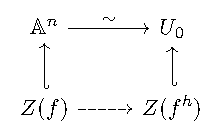
\includegraphics{lectures/5/pictures/cd_4.pdf}
		\end{center}

		Значит и соотвествующие открытые куски будут изоморфны. 
	\end{proof}

	\begin{example}
		Рассмотрим кривую в $C \subset \PP^2, \ C = Z(y^2 - xz)$. Рассмотрим отображения
		\[
			\PP^1 \to C,  (s : t) \mapsto (s^2 : st : t^2), \quad C \to \PP^2, \ (x : y : z) \mapsto \begin{cases} (x : y), & x \neq 0 \\ (y : z), & z \neq 0 \end{cases}.
		\]
		Видно, что эти отображения задают изомофизм $C$ и $\PP^1$. Но, однородные координатные кольца у этих многообразий~--- это $S(\PP^1) = \bk[x, y], \ S(C) = \bk[x, y, z]/(y^2 - xz)$, а они неизоморфны. 

		Это наводит нас на мысль о том, что для проективных многообразий нам нужен какой-то структурный инвариант сильнее. 
	\end{example}

	\subsection{Проективное замыкание аффинного многообразия}

	Пусть $T \subset \AA^n$~--- замкнутое подмножество, попробуем найти $\overline{T} \subset \PP^n$. 

	Первое, что приходит в голову~--- это просто взять гомогенизацию многочленов, которыми задаётся $T$, но это не всегда даст $\overline{T} \subset \PP^n$, что иллюстрируется следующим примером: 

	\begin{example}
		Пусть $T = Z(y - x^2, z - xy) \subset \AA^3$. Гомогенизируем все многочлены:  
		\[
			\PP^3 \supset Z(yw - x^2, zw - xy) \supsetneq Z(yw - x^2, zw - xy, y^2 - xz) \supset = \{ (st^2 : s^2 t : s^3 : t^3) \ \vert \ (s : t) \in \PP^1 \} T
.		\]
		С другой же стороны, 
		\[
			Z(yw - x^2, zw - xy) = \{ (st^2 : s^2 t : s^3 : t^3) \ \vert \ (s : t) \in \PP^1 \} \cup \{ (0 : 1 : 0 : 0) \}.
		\]
		Но, верно следующее 
		\begin{exercise}
			$\overline{T} = Z(\langle f^h \rangle_{f \in I(T) })$.
		\end{exercise}


	\textcolor{red}{Ээээ а что дальше???}	
	\end{example}

